\chapter{\label{chp:emshowers} Electromagnetic Showers in Liquid Argon}

As seen in Chapter~\ref{chp:sbn}, the detection and measurement of electron neutrinos in the SBN program is essential to its success.  Particularly important to detecting anomalous \nue signals is the rejection of photons from the electron candidate sample.  This chapter presents the first demonstration of two methods to reject photons from electron candidates using data from the \argoneut detector: topological separation and calorimetric separation.


\section{Electromagnetic Interactions in Argon}

An electromagnetic shower can originate in two ways. In the first, a high energy electron (produced as the outgoing lepton of a \nue interaction, for example $\nue + n \rightarrow e^− + p$) will travel through the argon freeing ionizaion electrons as it goes.  Eventually, the electron will scatter off of an argon nucleus. This rapid acceleration will cause the electron to emit a Bremsstrahlung gamma ray. This gamma can pair produce in the presence of an Argon nucleus or orbital electron, producing a secondary high energy electron and positron. The $e^+/e^−$ pair will then each produce a cascade, similar to the original electron, until the energy is depleted: electrons or positrons emitting Bremsstrahlung photons, and the photons pair producing or Compton scattering to produce more charged particles. Naturally, when all of the energy of the original particle has been exhausted by ionization of Argon from the charged particles, the shower will stop.

The second way to produce an electromagnetic shower originates with a high energy photon (an example source is from the decay of neutral pions: $\pi^0 \rightarrow \gamma \gamma$) instead of an electron. When the photon interacts, it most often pair produces near a nucleus (at energies typical of those photons produced by neutrino interactions). The process is identical to the electron-induced shower after the first particles, and so electromagnetic showers from photons and electrons are only different in the original particles.

Electron-induced and photon-induced showers have a distinguishing feature in that an electron shower has only one ionizing particle at the start of the shower. Photon-induced showers instead typically have two particles - an electron and positron. Because electrons and positrons are both minimally ionizing particles, the energy deposited in the first few centimeters of a photon induced shower will be approximately double that of an electron induced shower.  Once the electromagnetic cascade develops, the amount of ionization can no longer be used to distinguish electron- and photon-induced electromagnetic showers.

When a high energy photon is produced in an interaction in argon, it will travel some distance, typically less than 50cm in argon at 500 MeV, before it interacts with the argon and induces an electromagnetic shower.  Gammas are neutral particles, and they do not produce ionization until they interact via Compton Scattering or Pair Production. Thus there is often a visible gap between the origin of the gamma and the start of the electromagnetic shower. 

\begin{figure}[h!]
  \centering
  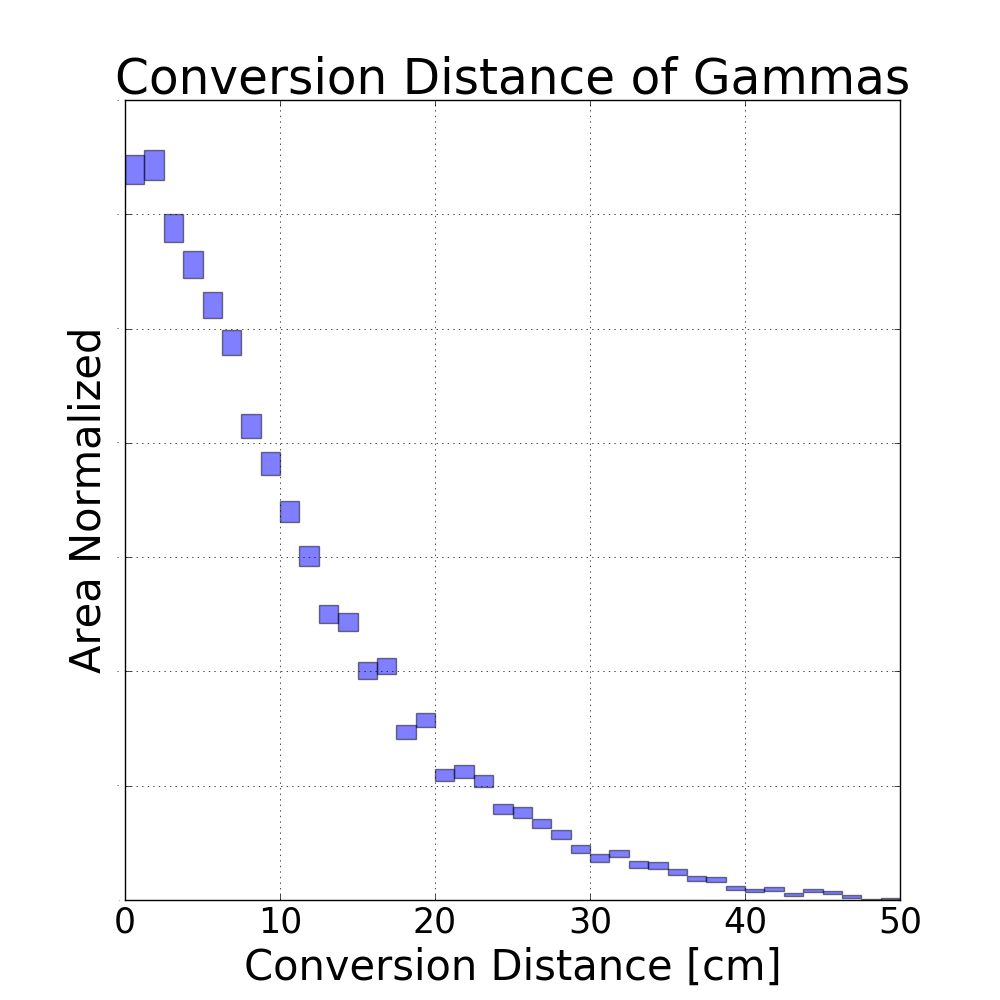
\includegraphics[width=0.5\textwidth]{emshower_figures/photon_conversion_dist.png}
  \caption[Photon Conversion Distance]{The conversion distance of each gamma in the Monte Carlo sample used for this analysis, which is about 7000 gammas in the energy range of several hundred MeV, as modeled by GEANT4 \cite{Agostinelli:2002hh}.  There are gammas that convert very close to the generation point (here, 7\% of the gammas convert within a centimeter).  The definition of ``too close'' depends on the analysis being performed, however, there will always be a fraction of gammas for which a topological based cut is insufficient to tag them as gammas. }
  \label{fig:photon_conversion_dist}
\end{figure}

The distance a gamma travels before interacting is stochastic, but for the energies typical of the gammas produced by neutrino interactions the distribution is shown in Figure \ref{fig:photon_conversion_dist}.  In the \argoneut detector, the minimal resolution of a gamma gap is approximately one wire spacing (4~mm). In neutrino interactions with hadronic activity at the vertex it is possible protons and pions can obscured the start of an electromagnetic shower.  In this case, gaps of even a few centimeters can be unidentifiable.

\begin{figure}[ht!]
  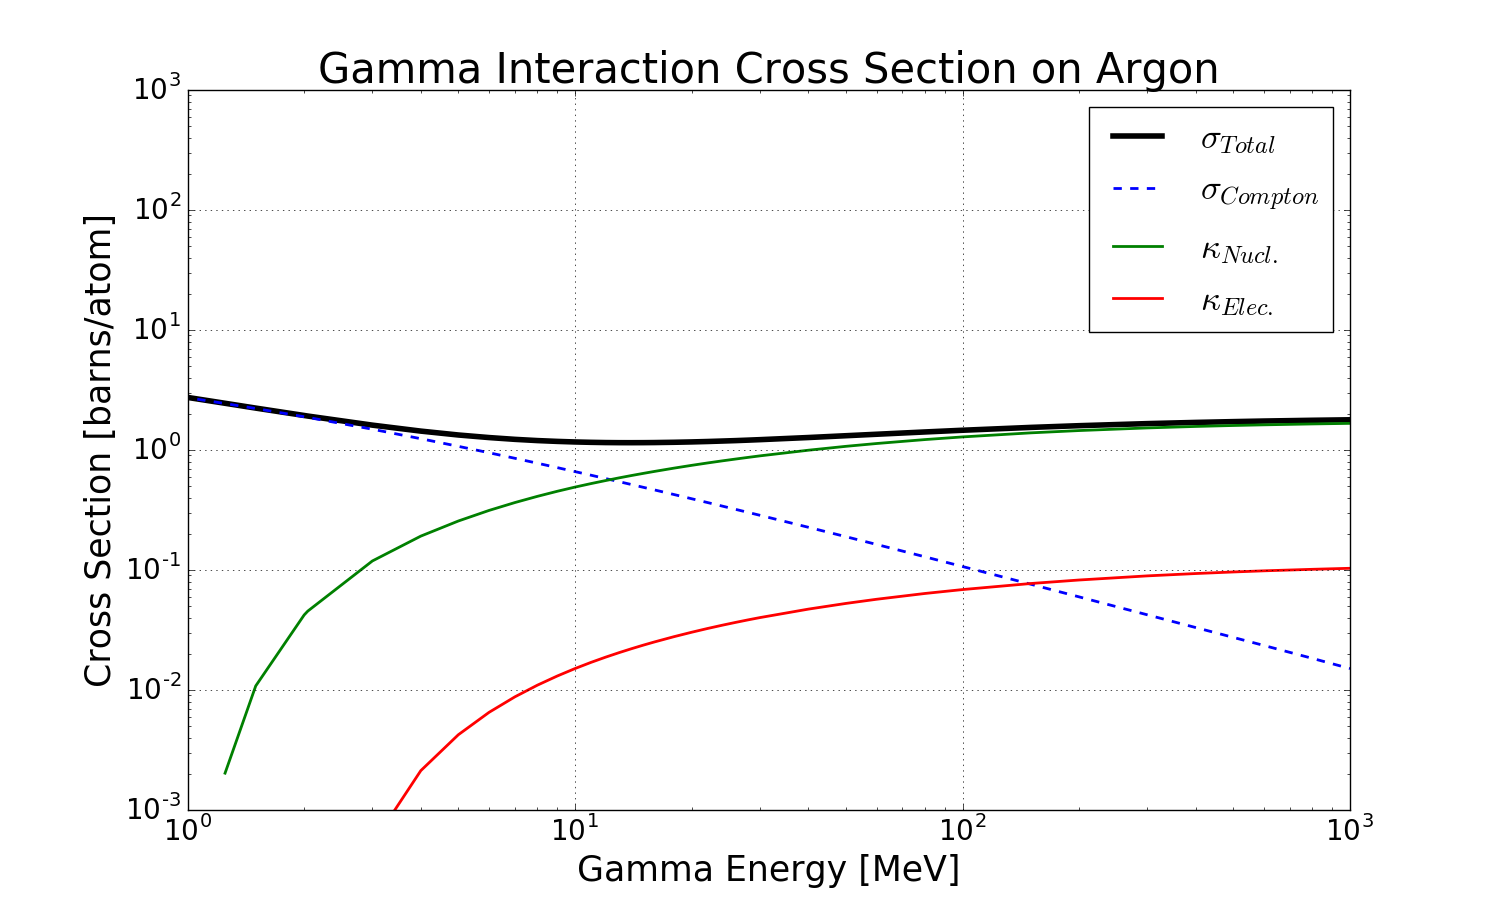
\includegraphics[width=\textwidth]{emshower_figures/photonCrossSection.png}
  \caption[Photon Cross Section on Argon]{\label{fig:gamma_xsec} The cross section of high energy gammas on Argon between 1 MeV and 1 GeV.  Here, $\kappa$ refers to the pair production cross section for the nuclear field and electron field.  Compton and pair production cross sections are balanced at just above 10 MeV.  Data are obtained from the Xcom database \cite{Xcom}.}
\end{figure}

The calorimetic separation of electrons and photons, using the amount of ionization measured at the start of the shower, depends on the photon interacting through pair production and not Compton scattering.  As seen in Figure~\ref{fig:gamma_xsec}, the scatter cross section of photons is dominated by pair production above 100 GeV, though the Compton cross section remains relevant up to 1 GeV of photon energy.  Figure~\ref{fig:relative_gamma_xsec} shows the relative probability that a photon will interact through either Compton or pair production channels.  Importantly, a photon that interacts through Compton scatter can not be distinguished via calorimetry from an electron.  Instead, only a topolgical separation can be used.  In most neutrino exeriments such as the SBN program \cite{Antonello:2015lea} and DUNE \cite{DUNE}, the high amounts of photons produced compared to expected electron neutrino events makes the fraction of Compton scatter photons a relevant background.  Therefore, both methods of separation are crucial.

\begin{figure}[ht!]
  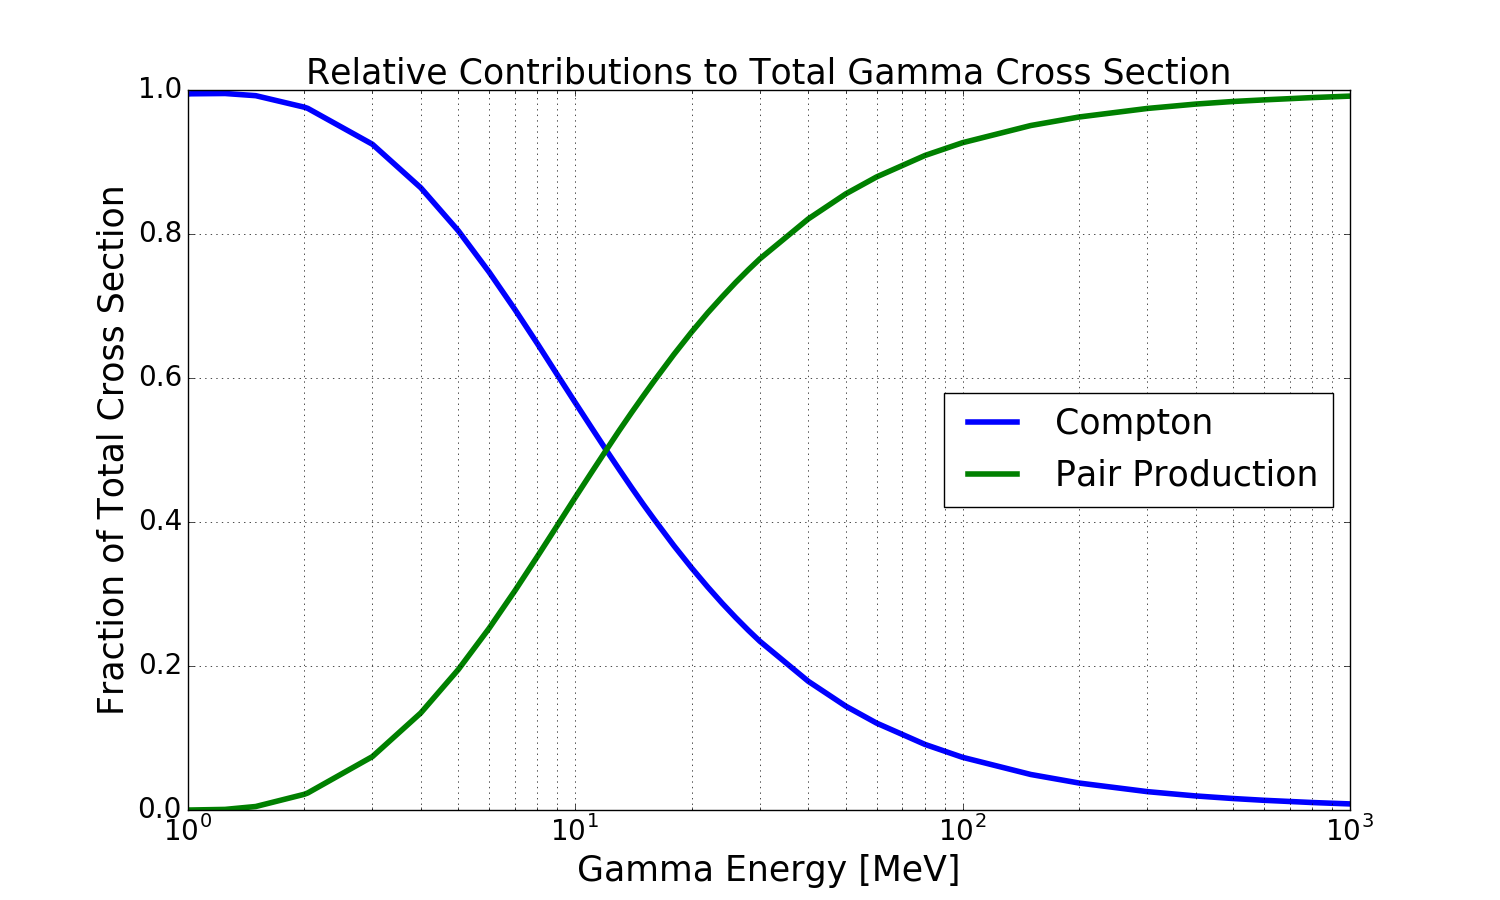
\includegraphics[width=\textwidth]{emshower_figures/relative_photonCrossSection.png}
  \caption[Comparison of Compton to Pair Production Cross Section]{\label{fig:relative_gamma_xsec} The cross section of high energy gammas on Argon between 1 MeV and 1 GeV.  Here, $\kappa$ refers to the pair production cross section for the nuclear field and electron field.  Compton and pair production cross sections are balanced at just above 10 MeV.  Data are obtained from the Xcom database \cite{Xcom}.}
\end{figure}


\subsection{Selection of Electromagnetic Showers in \argoneut}

To validate the separation of electromagnetic showers in \lartpcs, a study was performed using the neutrino events from the \argoneut detector to select samples of electron candidate and photon candidate events.  A sub-sample of the \argoneut data set containing electromagnetic showers is isolated first, and this sub-sample is used to select well defined electron and gamma events by visual scanning.

Selecting the sub-sample of electromagnetic showers is based on information from the 2-dimensional clusters of charge depositions (hits) in each wire plane. First, empty events and events with only track like particles in them are removed from the sample using an automated filter. This filter looked at two-dimensional clusters of hits made with the LArSoft package, and calculated several parameters of these clusters to differentiate between track-like and shower-like clusters \cite{Church:2013hea}. 

The two most successful metrics in separating tracks and showers for well clustered events are the principal eigenvalue of a principal component analysis (PCA), and a direction corrected hit density of the cluster.  Fig. \ref{fig:separation} shows these separation parameters obtained using Monte Carlo simulations of single electrons as a model for electromagnetic showers, and single muons and protons as a prototype for tracks. 
\begin{itemize}
  \item {\bf Principal Component Eigenvalue:} Principal component analysis takes a collection of N dimensional points and numerically finds the orthonormal coordinate system that best aligns to the data.  The goodness-of-fit metrics in PCA analysis are the eigenvalues of the transformation matrix between the initial coordinate system and the best fit.  In this analysis, we use the 2D reconstructed charge depositions (hits) in the wire-time views of the collection plane TPC data and performed principal component analysis on each cluster.  For track like particles, which have strong directionality, the first eigenvalue of the analysis is quite high, close to 1.  For shower like clusters, the direction of the shower and it's transverse direction are less obviously separated, and the principal eigenvalue is lower than 1.  For this analysis, a cut is made on the value of $log(1-E.V._{PCA}) > -5$ as seen in figure~\ref{fig:separation}.  This corresponds to rejecting all clusters that have a principal eigenvalue greater than 0.999.
  \item{\bf Direction Corrected Hit Density:}  A showering event is defined by the fact that there is significant activity in the TPC that is resolved away from the primary axis of the particle.  That is, a shower has many hits reconstructed as it travels through the TPC, whereas a track generally has one charge deposition detected per step through the TPC.  Measuring the hit density, defined as hits per unit distance, along a particle can thus discriminate between tracks and showers.  Since hits are only reconstructed on wires, and tracks and showers need not be perpendicular to the wires, the hit density is corrected to account for the fact that high angle tracks and showers (more parallel to the wires) have relatively fewer hits reconstructed.  In this analysis, events with a corrected hit density greater than 1.5 are kept, and the relative distributions for single tracks and showers are shown in figure~\ref{fig:separation}.
 \end{itemize}

\begin{figure}[ht]
\centering
\includegraphics[width=0.45\textwidth]{emshower_figures/modhitdensarea_proper.pdf}
\includegraphics[width=0.45\textwidth]{emshower_figures/princcomp_area_proper.pdf}
\caption[Track/Shower Discrimination Metrics]{\label{fig:separation} ``Modified hit density'' and Principal Component Eigenvalue calculated for single electron showers(red) and muon tracks (blue).}
\end{figure}

An additional requirement is that a shower-like cluster in on plane should correspond to an analogous cluster in the second plane. This removed spurious tags due to wire noise or other sources.




Finally, an additional set of cuts is applied using all of the hits in a single view in an event as a single cluster. These cut remove high-energy Deep Inelastic Scatter events or cosmic events which resulted in too much total charge in an event. 

This procedure resulted in sample of ArgoNeuT events that contained mostly EM-shower events, from which the final electron and gamma samples are selected.

Unless there is other activity in the detector at the location of gamma production, the gap is impossible to detect.  Therefore, two types of events are classified as gamma candidates, based on the observation of charged protons or pions at a neutrino interaction vertex: electromagnetic showers pointing back to charged particle activity at a vertex with hadronic interaction, and Neutral Current $\pi^0$ events where two electromagnetic showers project back to a common point.  In the second case, hadronic activity at the vertex is allowable but not required.  Examples of both types of gamma interactions are shown in Figure~\ref{fig:photons}.  Gammas that are unable to be positively identified purely through topological considerations - if, for example, the electromagnetic shower is the only activity in the detector - are not used in this analysis.



\begin{figure}[ht]
\centering
\includegraphics[width=\textwidth]{emshower_figures/PhotonEvents.pdf}
\caption[Photon Events in \argoneut]{\label{fig:photons} Examples of gamma candidate events.  The top row are the induction views and the bottom row are the collection views of two events. In both cases, the key identifying feature is the gap between the showers and the other activity to which they point backwards.  In the (bottom) collection planes, there is a block of 5 wires that are inactive.}
\end{figure}

For a sample of electrons, this analysis targeted electron neutrino events as the electron shower candidates.  To maximize purity, an electromagnetic shower is selected as an electron candidate only in events that also exhibited hadronic activity at the vertex {\em without} the presence of a gap between the shower and other particles.  In addition, events with a track like particle matched to a muon in the MINOS near detector are rejected.  This ensures that the contamination from $\nu_\mu$ Charged Current events with high Bremsstrahlung activity is negligible.  Examples of electron candidates are shown in Figure~\ref{fig:electrons}. In total, 37 electron candidate showers and 274 gamma candidate showers are selected for this analysis.



\begin{figure}[ht]
\centering
\includegraphics[width=\textwidth]{emshower_figures/ElectronEvents.pdf}
\caption[Electron Candidate Events in \argoneut]{\label{fig:electrons} Examples of $\nu_e \rightarrow e$~CC events.  The top row are the induction views and the bottom row are the collection views of two events. In both cases, there is no observable gap between the shower and the hadronic activity.In the (bottom) collection planes, there is a block of 5 wires that are inactive due to a bad electronics connection in the detector.}
\end{figure}


\section{Reconstructing Electromagnetic Showers in \lartpcs}

To reconstruct electromagnetic showers in \lartpcs, a procedure described in Section~\ref{sec:lartpc_reconstruction} is applied.  In general, the raw data from the detector must be deconvolved to mitigate noise sources, and a peak finding algorithm is applied to the signal from each wire to find charge depositions, known as hits. The integral of the ADC count in each hit is used to calculate the charge $dQ$ using an (ADC$\times$Timetick)/Coulomb conversion constant.  The constants are obtained using the procedure described in \ref{subsec:lartpc_calibration}, which follows the procedure in \cite{Anderson:2012mra}.

The most difficult step in the reconstruction of electromagnetic showers, by far, is deciding which hits in an interaction are associated with the shower. For the events selected to demonstrate electon/gamma separation, the hits were assembled into appropriate clusters manually.

In order to measure dE/dx correctly, it is extremely important to precisely determine the start point and direction of the shower. In particular, the start point and direction are needed to measure the {\em first} several centimeters of the shower before the development of the electromagnetic cascade. Once the shower develops, the electron and gamma populations become significantly less distinguishable (see Section \ref{sec:dedx_calcs}). 


\subsection{Reconstruction Algorithms}

\begin{figure}[h!]
  \centering
  \includegraphics[width=\textwidth]{emshower_figures/iterative_start_point.pdf}
  \caption[Diagram of the 3D start point algorithm.]{Diagram of the 3D start point algorithm.}
  \label{fig:iterative_start_point}
\end{figure}

The 3D start point is initially calculated from the intersection point of the wires where the two 2D start points are found and their position in the drift time coordinate.  The start point in 3D is improved using an iterative algorithm, and illustrated in Figure \ref{fig:iterative_start_point}.

An initial guess, the point in black, is made for the start point based on the 2D start points (yellow stars in each plane).  The start point in 3D is projected into each plane, and the error in the 3D start point is the sum (over each plane) of the distance between the true start point in each plane and the projection of the 3D point.  Six additional points, along the detector coordinates (in the $\pm$ x, y, and z directions), are also projected into each plane, and the error of each point is computed similarly (black dashed lines show the distance between projection and true start point).  The point with the smallest summed error is chosen as the better 3D start point, and the algorithm makes an additional six guesses around it.  If the central point (in black) is chosen as the best fit point, the distance the other 6 points are offset from it is decreased and the algorithm repeats.  This procedure is repeated until the algorithm can no longer improve the accuracy of the 3D start point.  The initial offset from the central point for the 6 auxiliary points is 5 centimeters, and it decreases by 2\% for each successful iteration.  As seen in Figure~\ref{fig:shower_reco}, the 3D start point resolution is generally better than 1 cm.

\begin{figure}[h!]
  \centering
  \includegraphics[width=\textwidth]{emshower_figures/iterative_start_dir.pdf}
  \caption[Diagram of the 3D start direction algorithm.]{Diagram of the 3D start direction algorithm.}
  \label{fig:iterative_start_dir}
\end{figure}


Similar to the 3D start point, the 3D axis is computed using an iterative projection matching algorithm.  The standard TPC trigonometric formula is used to compute an approximate 3D axis based on the angle of each shower in the collection and induction plane:

\begin{align}
  \theta &= \text{arccos}\frac{m}{\sqrt{l^2 + m^2 + n^2}}, \\
  \phi &= \text{arctan}\left(\frac{n}{l}\right) 
\end{align}
where
\begin{align}
l &= sign(t_{end} - t_{start}), \\
m &= \frac{1}{2 \text{sin}(\alpha)}\left(\frac{1}{\Omega_0} - \frac{1}{\Omega_1}\right), \\
n &= \frac{1}{2 \text{cos}(\alpha)}\left(\frac{1}{\Omega_0} + \frac{1}{\Omega_1}\right).
\end{align}

Here, $\theta$ represents the polar angle in 3D with respect to the z axis (approximately the beam direction).  $\phi$ is the azimuthal angle in the x-z plane, with $\phi$ = 0 along the z axis, and  $\alpha$ is the angle of the wire planes with respect to the vertical direction, which in ArgoNeuT is 60 degrees.  $\Omega_0$ and $\Omega_1$ are the tangents of the 2D angles of the shower measured in each plane.  $t_{start}$ and $t_{end}$ are the start and end points of the cluster, such that $l$ is positive if the shower points away from the wires and positive the shower points towards the wires.

\begin{figure}[p]
   \centering
   
   % 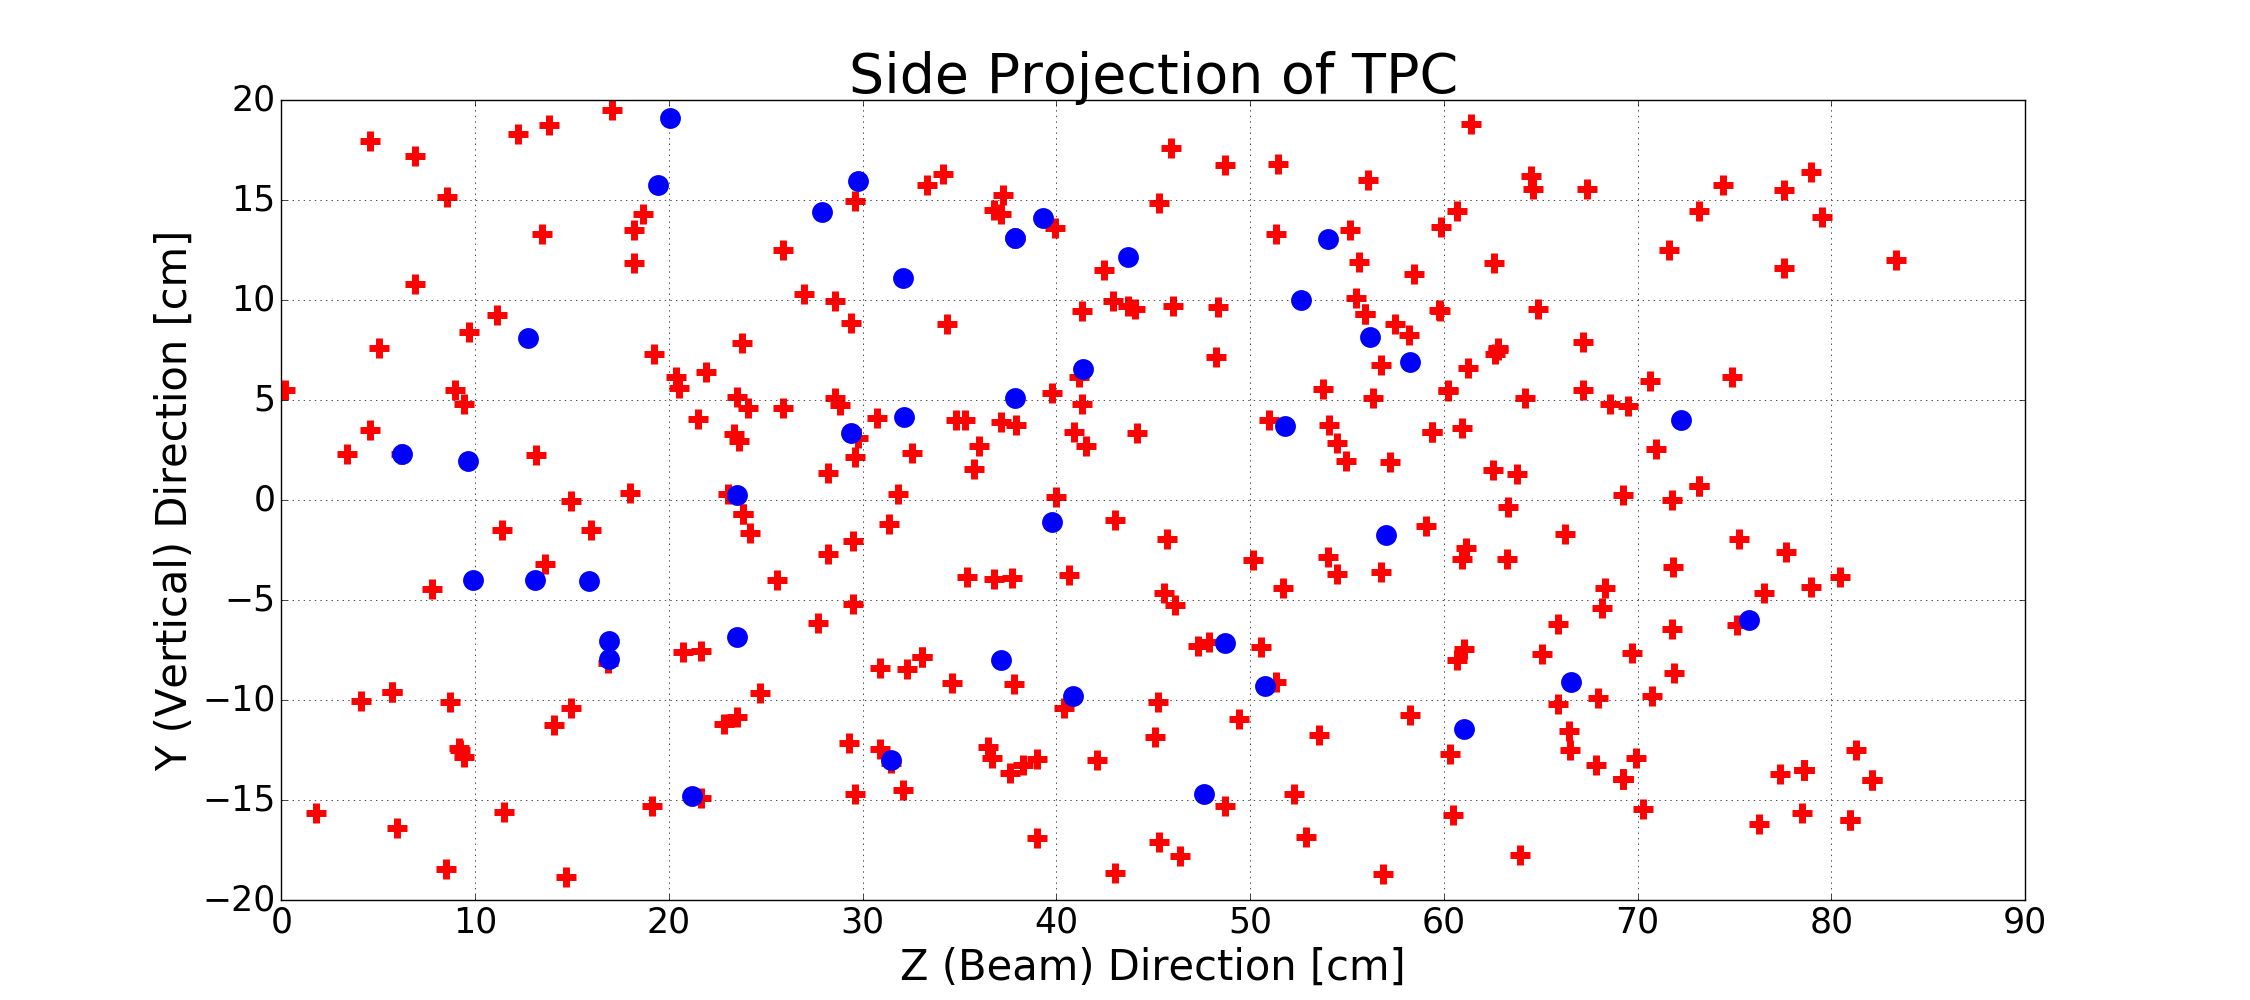
\includegraphics[width=0.9\textwidth]{emshower_figures/yz_projection.png}
   % 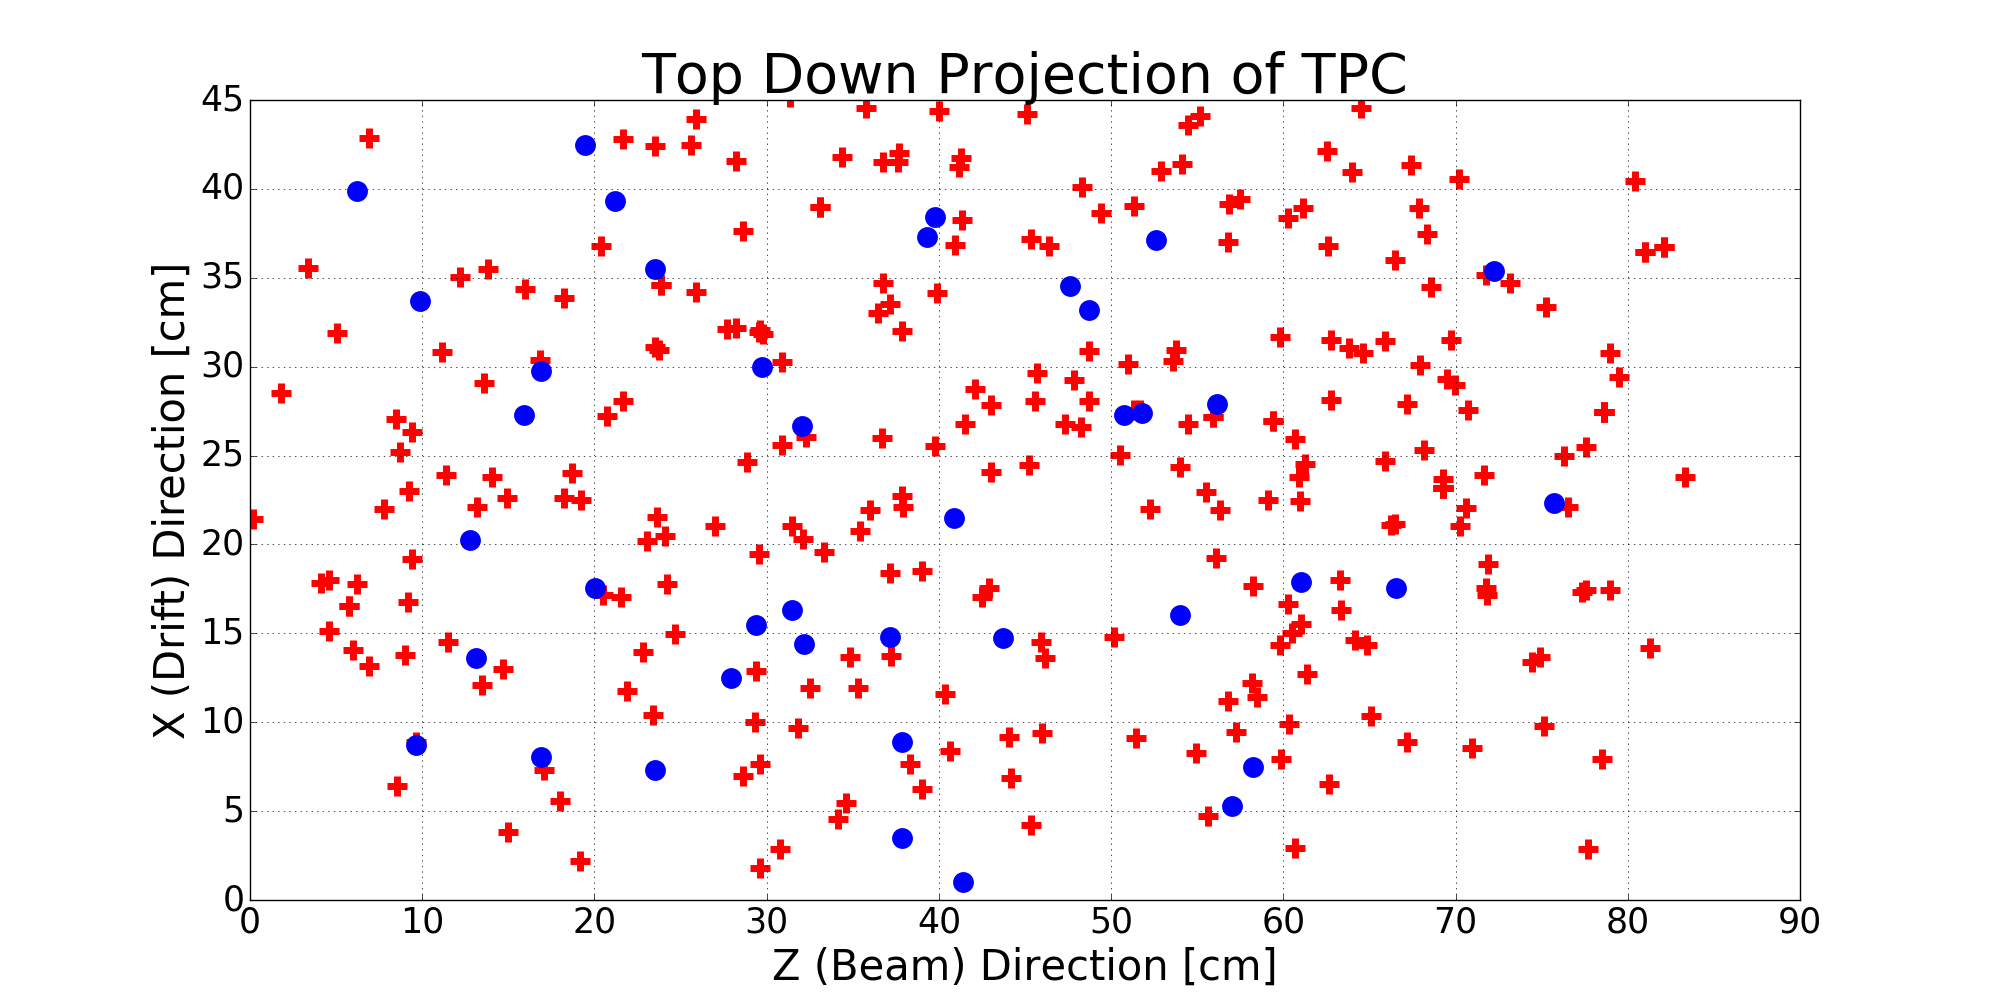
\includegraphics[width=0.9\textwidth]{emshower_figures/xz_projection.png}
   % 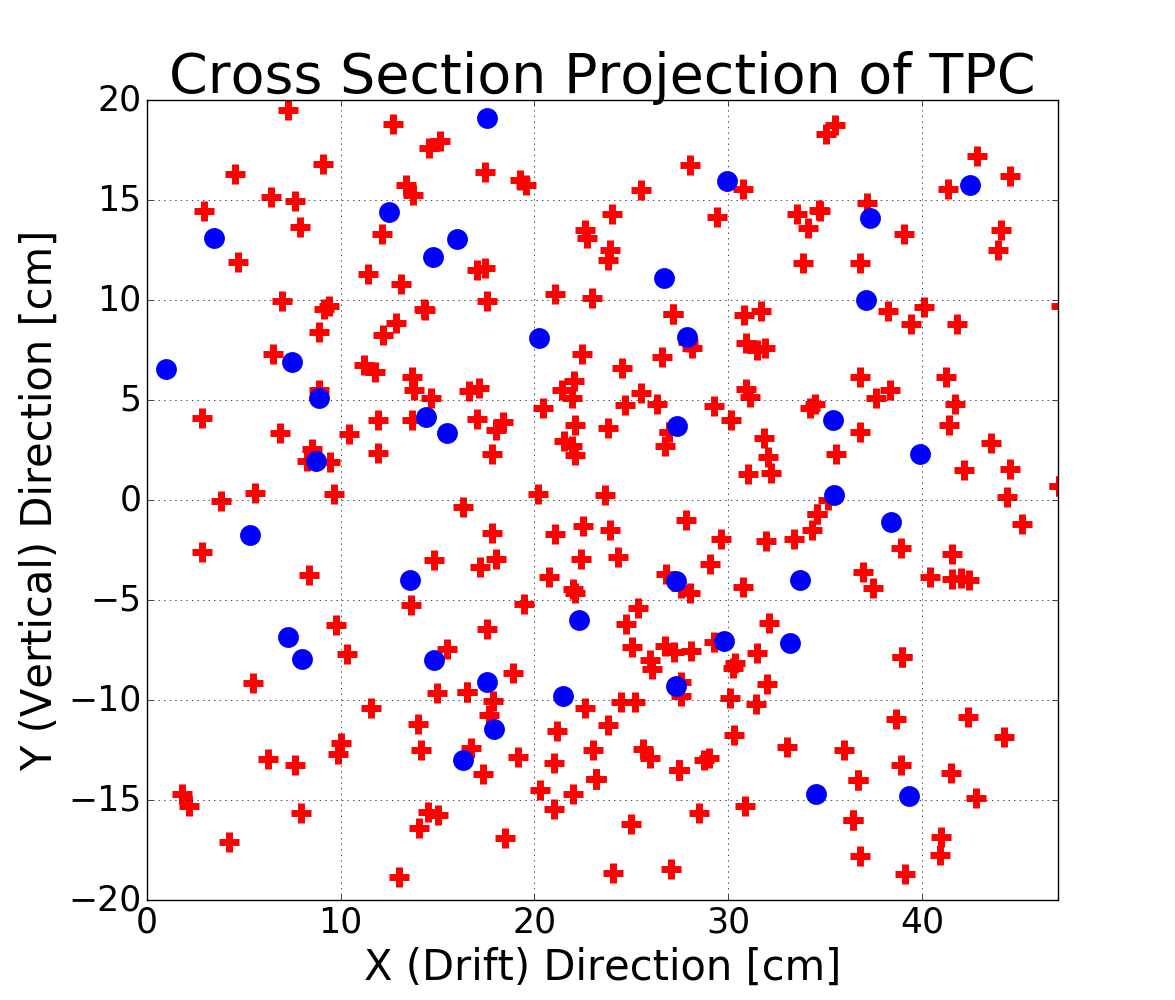
\includegraphics[width=0.9\textwidth]{emshower_figures/xy_projection.png}
   % 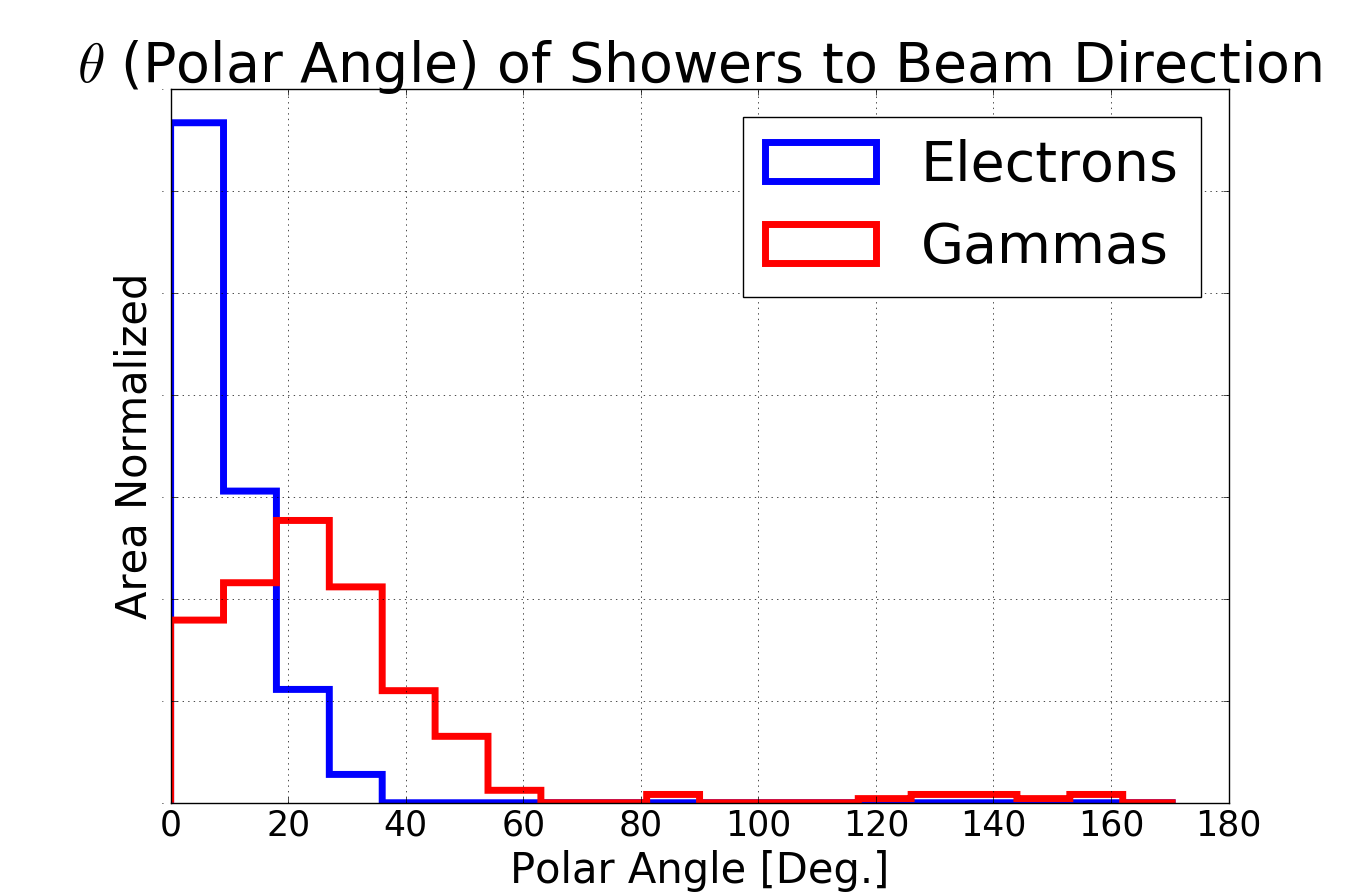
\includegraphics[width=0.9\textwidth]{emshower_figures/theta_distribution.png}
   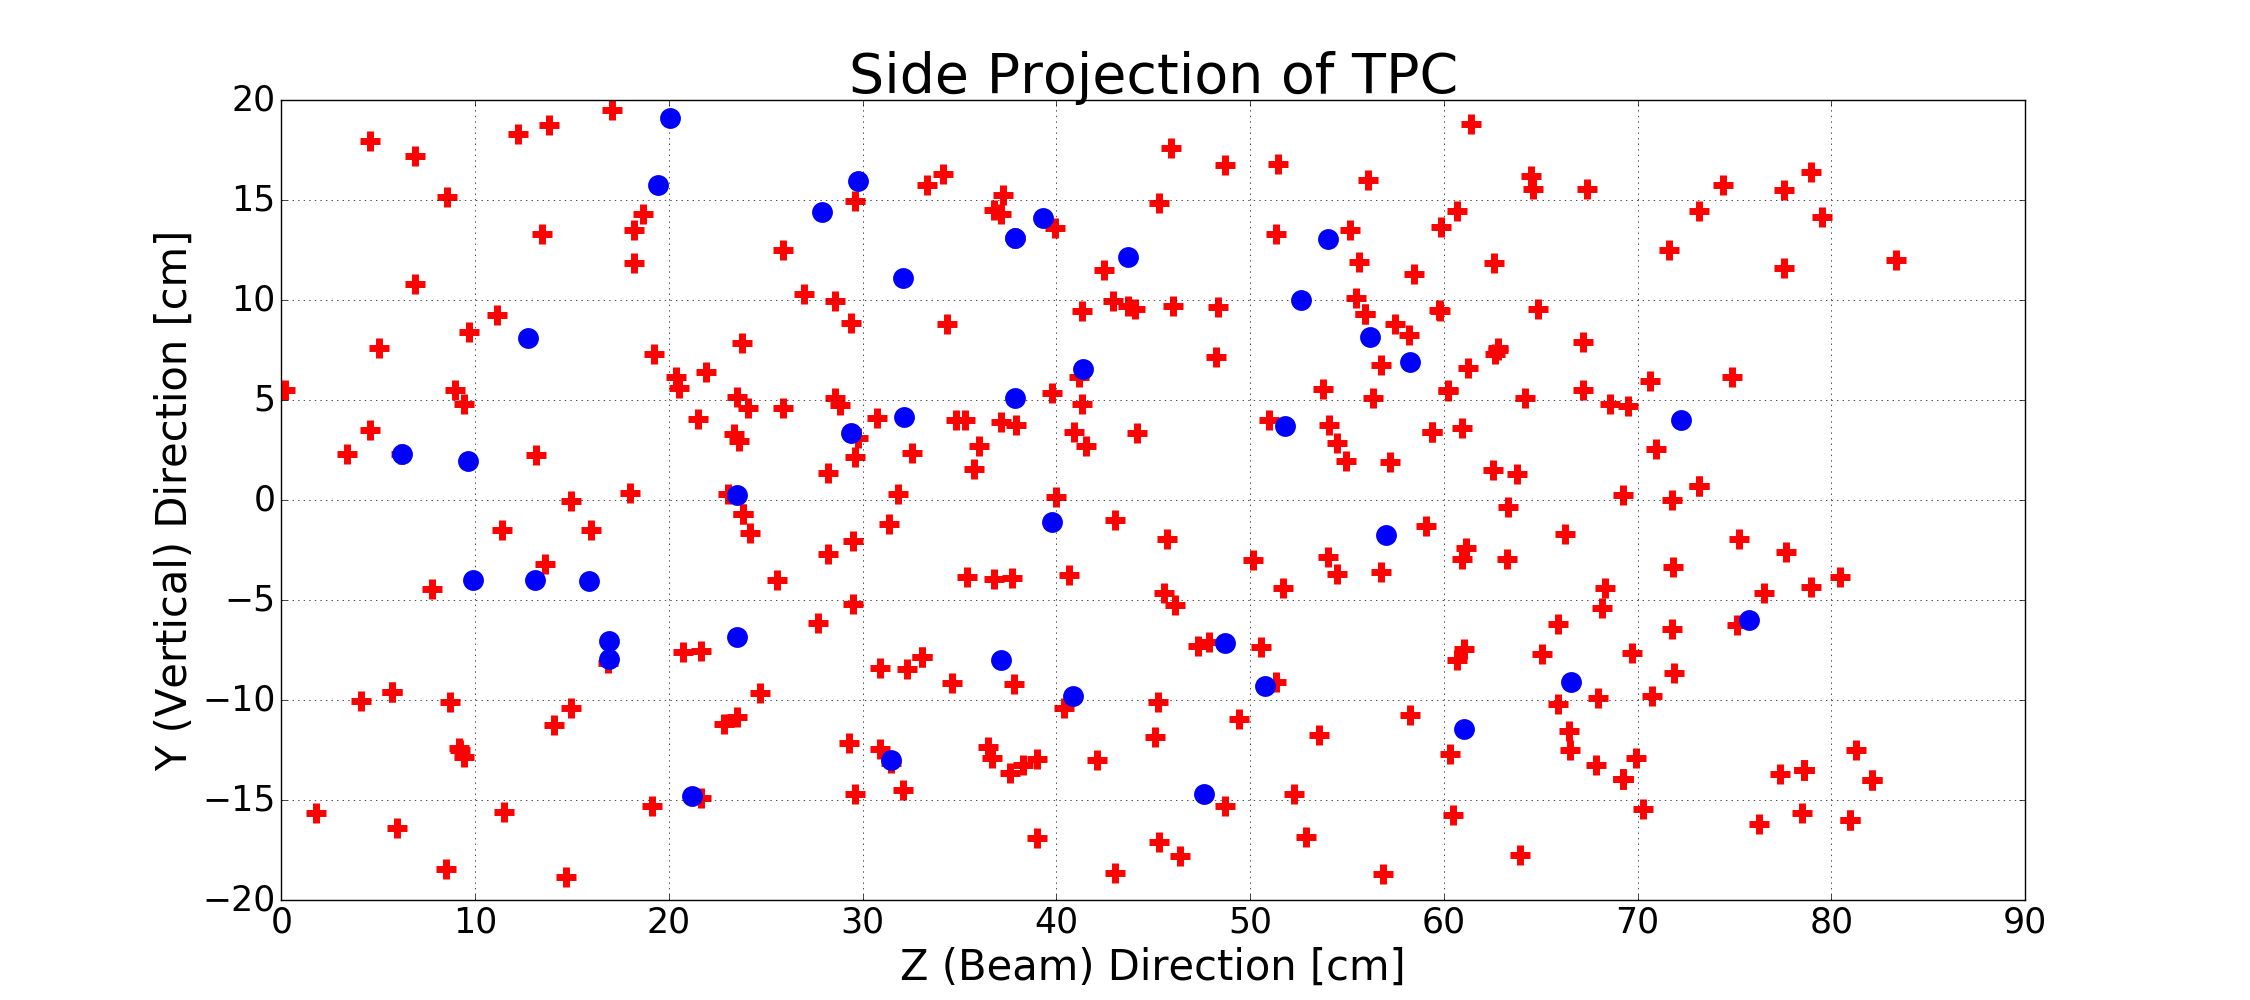
\includegraphics[height=2in]{emshower_figures/yz_projection.png}
   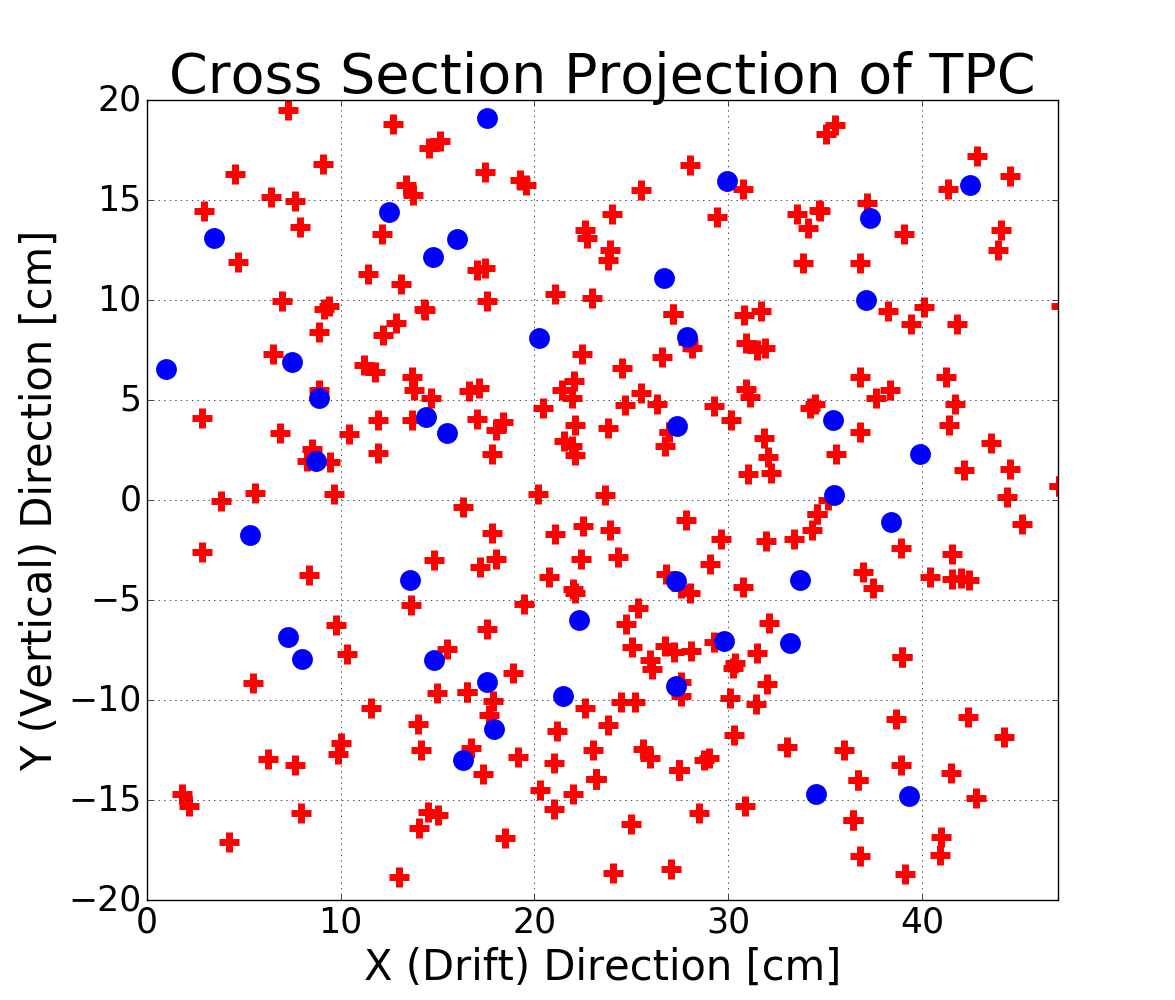
\includegraphics[height=2in]{emshower_figures/xy_projection.png}
   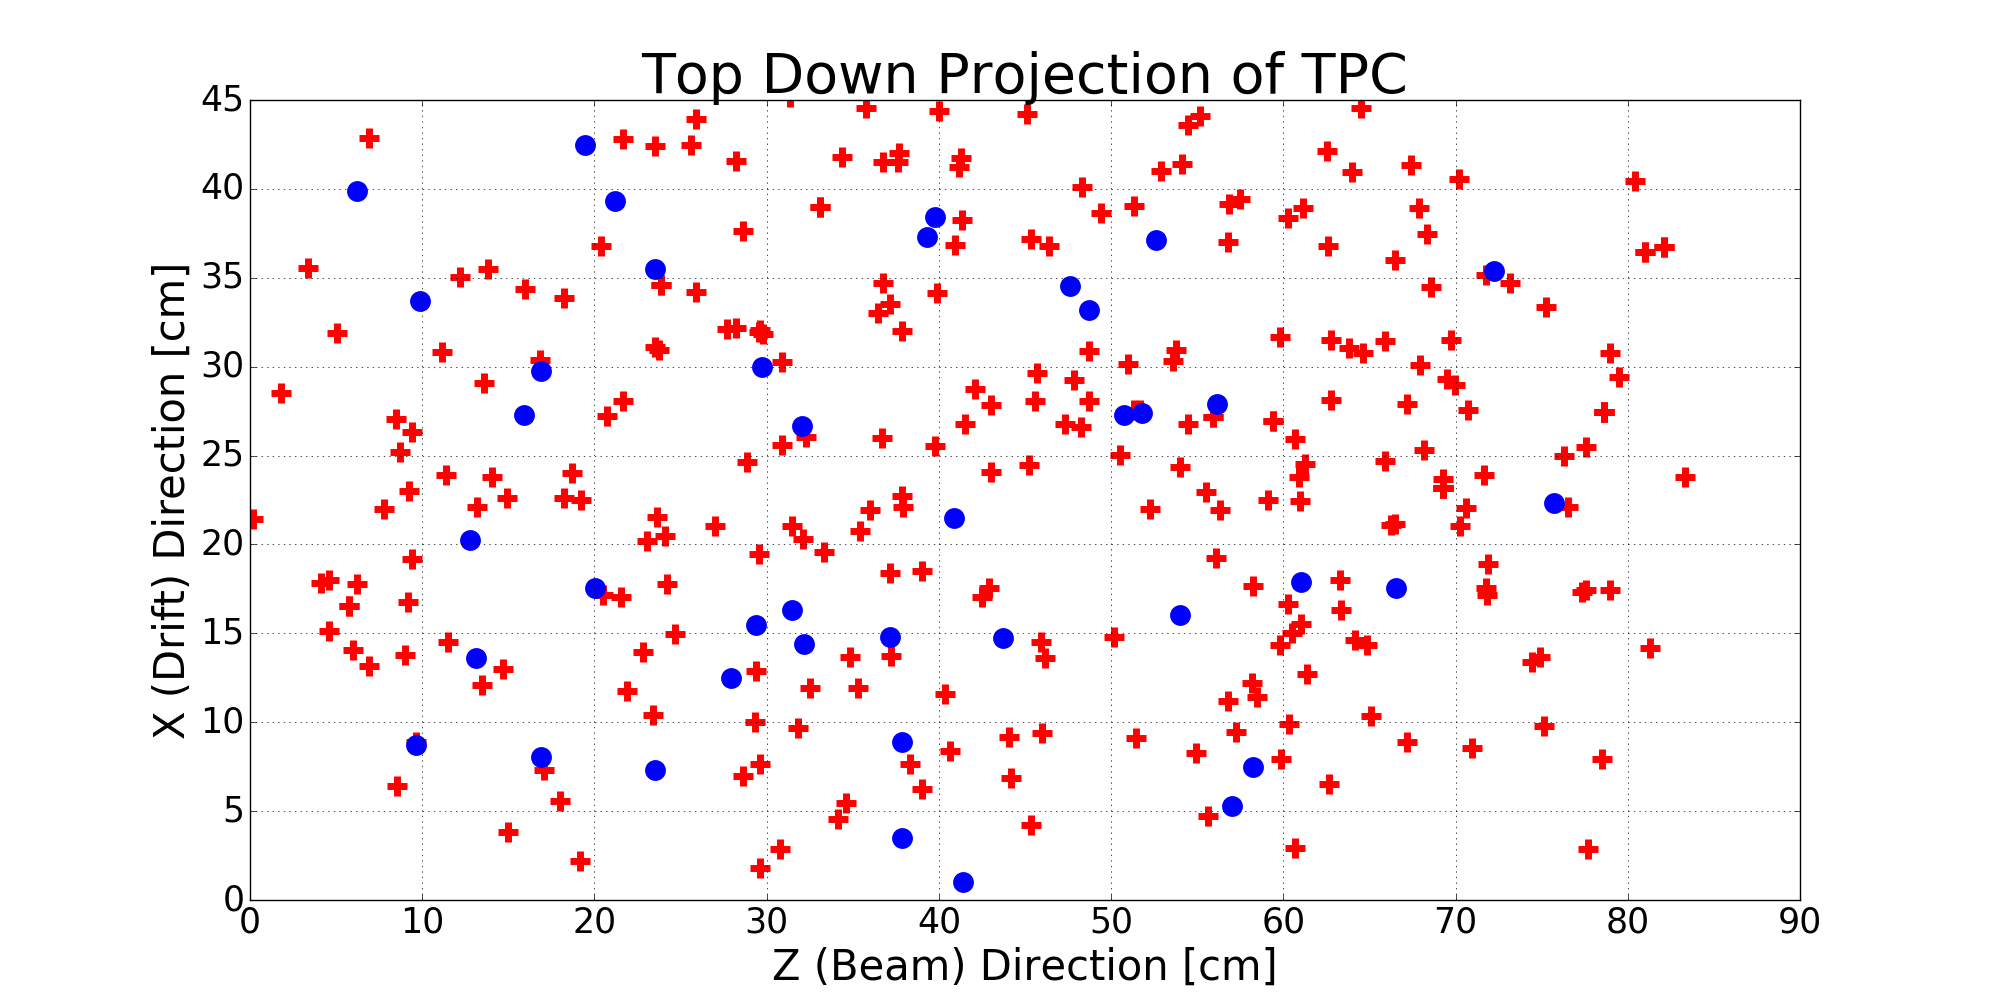
\includegraphics[height=2in]{emshower_figures/xz_projection.png}
   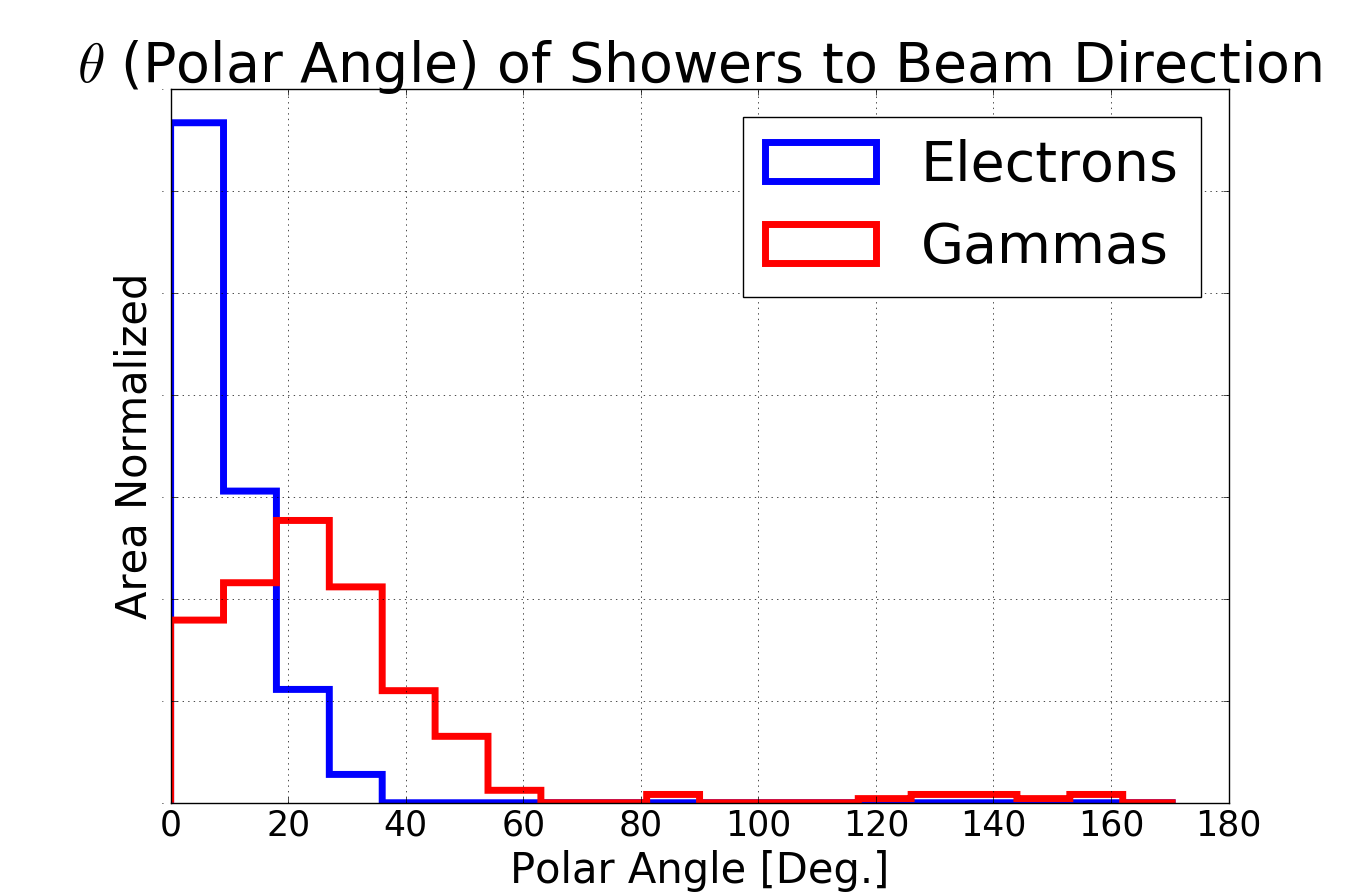
\includegraphics[height=2in]{emshower_figures/theta_distribution.png}
   \caption[Vertex Distributions of Electromagnetic Showers.]{The vertexes of electron candidates (blue circles) and gamma candidates (red plus signs) in the Z-Y, Z-X, and X-Y projections, as well as the distribution of the polar angle of events with respect to the Z direction (approximately the beam direction).  The electron sample is very forward going, and the gamma sample has a wider distribution of angles. }
   \label{fig:geomety_dists}
 \end{figure} 

\begin{figure}[p]
   
   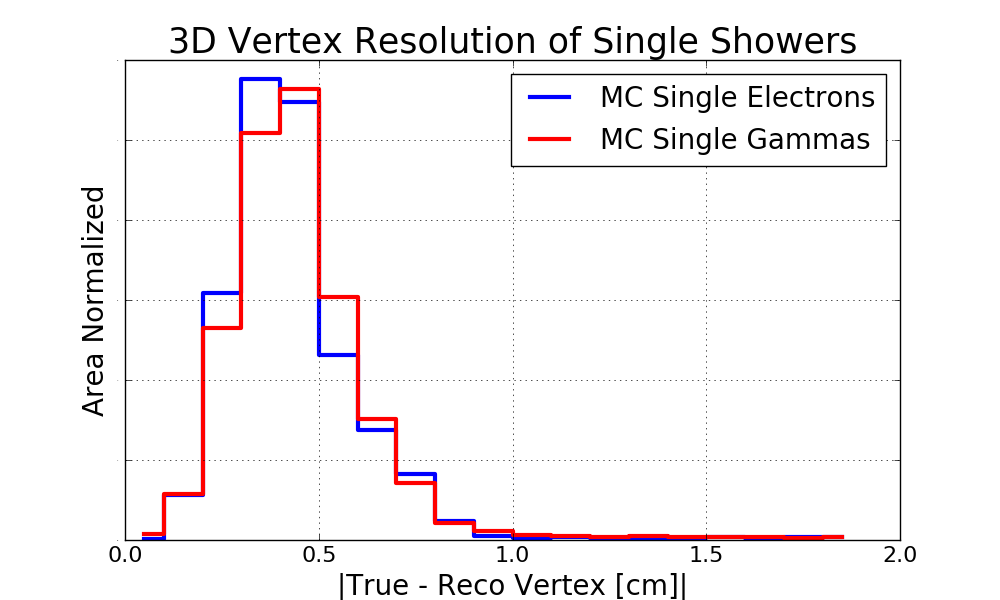
\includegraphics[width=0.45\textwidth]{emshower_figures/3d_resolution.png}
   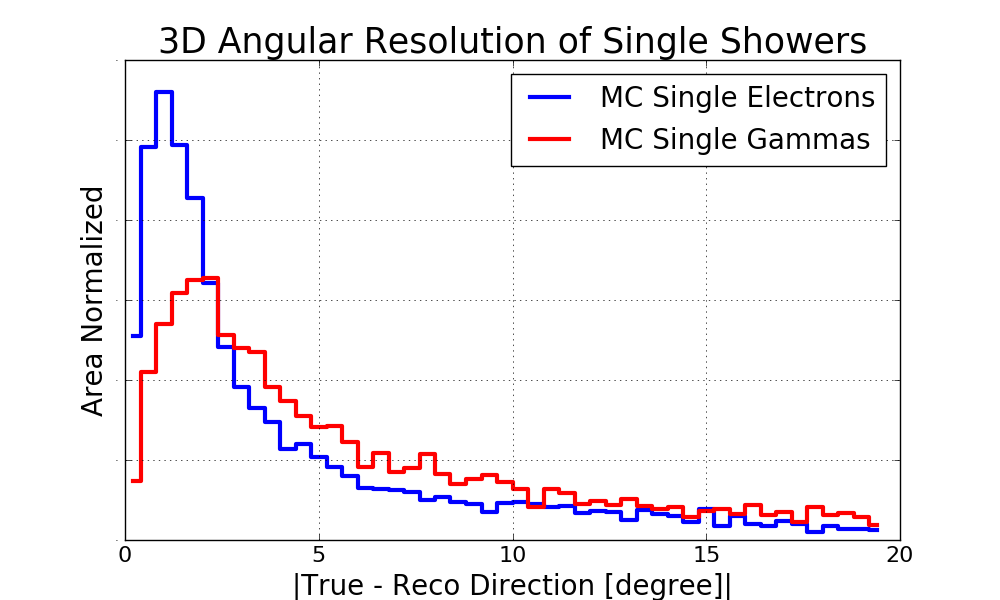
\includegraphics[width=0.45\textwidth]{emshower_figures/AngularResolution.png}
   \caption[Resolution of Electromagnetic Showers]{The calculated resolution of the 3D start point (left) and angular resolution (right) for single electromagnetic showers generated with the LArSoft package.  The angular resolution for gammas is slightly worse than for electrons because the gamma sample is at lower energy, and hence has fewer depositions (hits) in the TPC.}
   \label{fig:shower_reco}
 \end{figure} 


The reconstructed 3D axis is then projected into each plane, and the slope (in 2D) is compared against the slope of the electromagnetic showers in each plane.  Based upon the quality of the match between the projection and the 2D slopes, the 3D axis is adjusted until the best fit is obtained - see Figure~\ref{fig:iterative_start_dir}.  An initial guess, the arrow in black, is made for the start direction based on the 2D start directions (red arrows in each plane).  The start direction in 3D is projected into each plane, and the error in the 3D start direction is calculated.  An additional set of 3D directions (gray arrows) are also projected into each plane.  If the central direction (in black) is chosen as the best fit direction, the angular separation between it and the other (gray) directions is decreased and the algorithm repeats.  This procedure is repeated until the algorithm can no longer improve the accuracy of the 3D start direction.

The angular resolution for electromagnetic showers, shown in Figure~\ref{fig:shower_reco}, is generally quite good though (better than 5 degrees) there is a substantial tail.  However, for this analysis, the poor resolution in a few measurements of the 3D axis has a minimal effect on the dE/dx calculation.  This is due to the fact that the majority of the events are forward going, as shown in Figure \ref{fig:geomety_dists}.  Therefore a moderate uncertainty in the 3D angle leads to only a small uncertainty in the effective wire pitch, described below, and a small uncertainty in dE/dx.


For the calorimetric separation of electrons and gamma to succeed, the dE/dx metric must be well reconstructed. As the charge depositions are measured discretely in 2D on single wires, in each of the wire planes we use the 3D axis of the shower to calculate an ``effective'' wire pitch between hits.  This effective pitch is, in other words, the real distance in the TPC that a particle travels between its two projections (hits) on adjacent wires. Figure \ref{fig:effective_pitch} shows the distributions of effective pitches for the electron and gamma samples.  In the calculation of dE/dx, the effective pitch is used as the estimate of `dx'.

\begin{figure}[p]
  \centering
  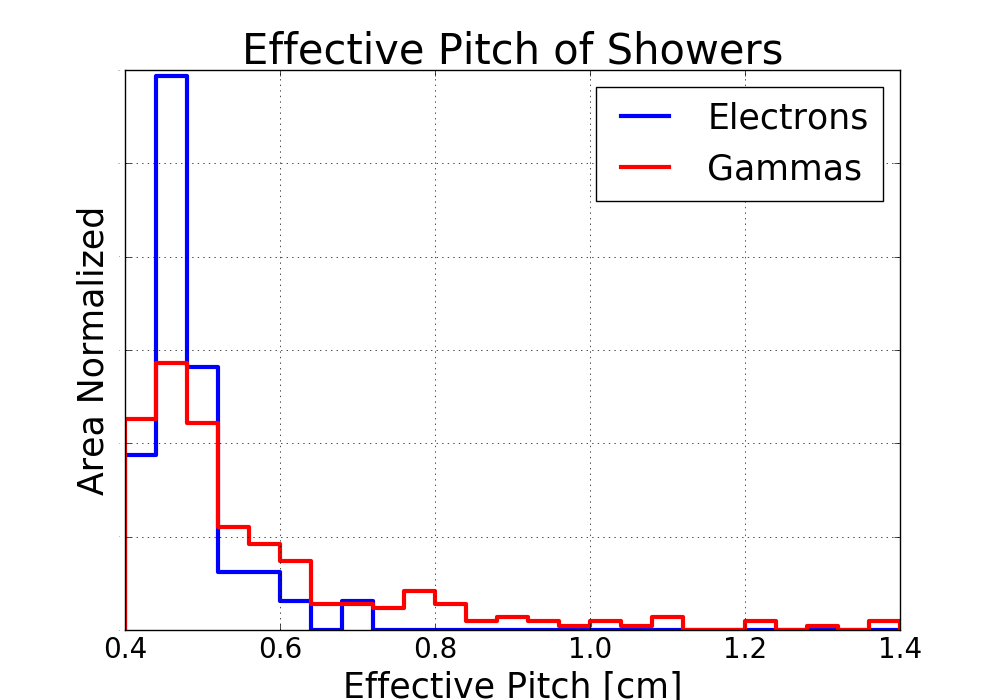
\includegraphics[width=0.5\textwidth]{emshower_figures/effective_pitch.png}
  \caption[Effective Pitch]{The effective pitch for the electron and gamma samples used in this analysis.  The effective pitch is a measure of how far a particle travels between depositions of charge recorded on adjacent wires.  The effective pitch is at least the wire spacing, which is 0.4 cm in ArgoNeuT.  The gamma distribution shows a slightly higher effective pitch, which is expected from Figure \ref{fig:geomety_dists} showing that the gammas are at slightly higher angles to the wire planes than the electron sample.}
  \label{fig:effective_pitch}
\end{figure}

An valuable cross-check of this sample of events is the distribution of every dE/dx deposition measured at the start of the shower, from all the events in the selected sample.  Figure~\ref{fig:photon_landau} shows this distribution for the gamma sample, along with the corresponding estimate from the Monte Carlo simulation.  Since the gamma sample is produced entirely by selecting showers with a displaced vertex, for this work the purity of the gamma sample is taken to be 100\%.

\begin{figure}[p]
  \centering
  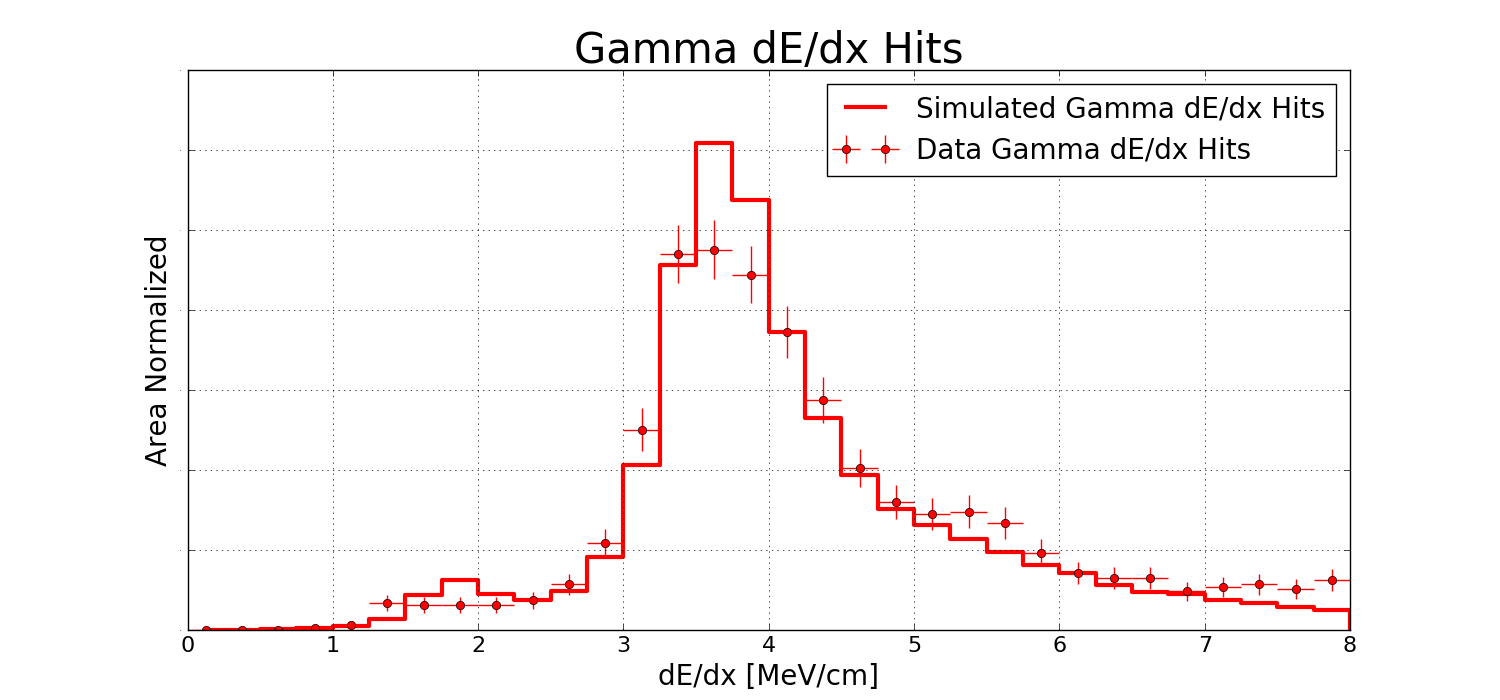
\includegraphics[width=0.8\textwidth]{emshower_figures/photons_landau.png}
  \caption[Photon Landau Distribution]{Distribution of dE/dx for all hits at the start of the shower for the gamma sample.  Unlike the aggregate measure of dE/dx, this plot uses the Modified Box Model \cite{Acciarri:2013met}.}
  \label{fig:photon_landau}
 \end{figure} 

\begin{figure}[p]
  \centering
   
  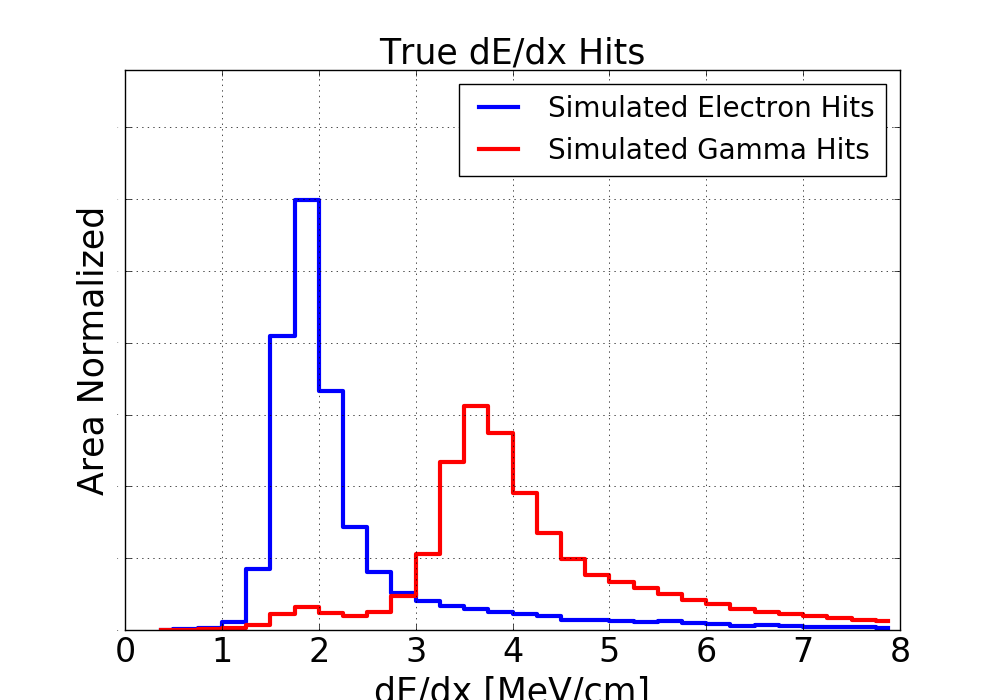
\includegraphics[width=0.8\textwidth]{emshower_figures/mcLandaus.png}
  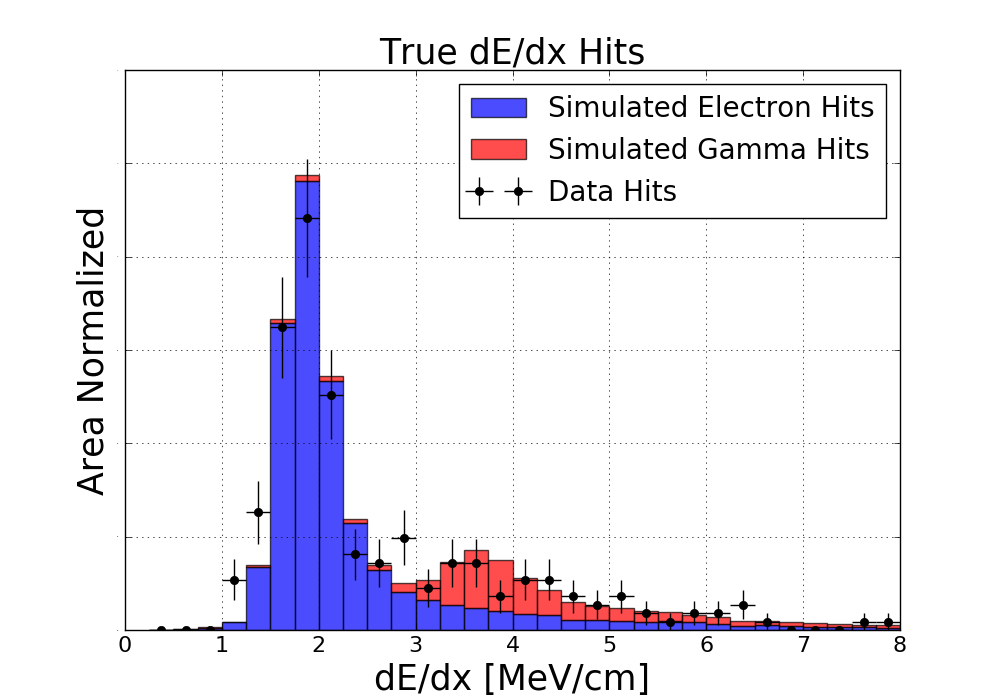
\includegraphics[width=0.8\textwidth]{emshower_figures/fitted_electron_distribution.png}
  \caption[Estimate of Photon Contamination in Electron Sample]{(Top) Normalized Monte Carlo distribution of dE/dx for all hits in a pure electron and pure gamma sample.  (Bottom) All dE/dx hits from the electron candidate sample, compared to a sample of Monte Carlo comprised of 80\% electrons and 20\% gamma.}
  \label{fig:electron_landau}
\end{figure} 




\begin{figure}[p]
  \centering
  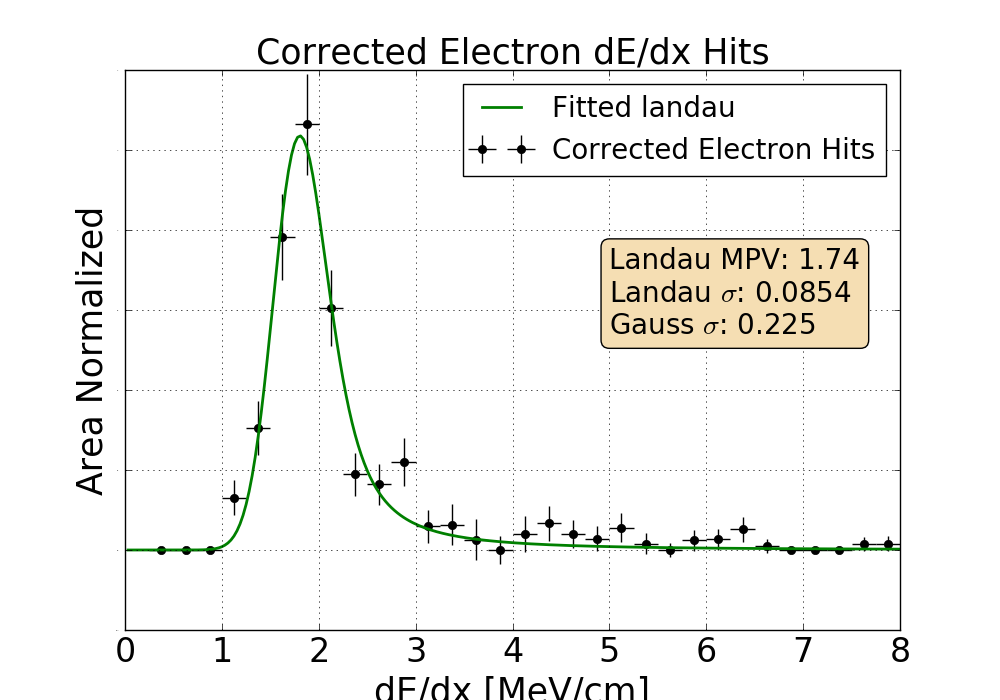
\includegraphics[width=\textwidth]{emshower_figures/fitted_electron_landau.png}
  \includegraphics[width=\textwidth]{emshower_figures/mpv_electrons.pdf}
  \caption[Electron Landau Distribution]{(Left) Background subtracted distribution of the hits at the start of the electron showers, with a fitted Gaussian-convolved Landau .  (Right) Most probable value of ionization as a function of momentum for particles traversing liquid argon.  For electrons above 100 MeV/c, as this sample is, the theoretical expectation of the most probable ionization is 1.77 MeV/cm.  This is in good agreement with the fitted value of 1.74 MeV/cm.}
  \label{fig:mpv_electrons}
 \end{figure} 



For the electron sample, we can not assume that the purity of the sample is 100\% based on topology alone.  As seen in Figure~\ref{fig:photon_conversion_dist}, a non-negligible amount of gammas will convert at a sufficiently short distance that they will get selected as electrons in a topological based cut.  Hadronic activity at the vertex can also obscure the presence of a gap from a gamma.  Therefore, the distribution of electron-like dE/dx hits analogous to Figure~\ref{fig:photon_landau} is expected to be modeled by a combination of electron and gamma showers in Monte Carlo.

In Figure~\ref{fig:electron_landau}, the Monte Carlo histograms for each dE/dx hit for electrons and gammas are shown.  These two distributions are used to fit to the equivalent distribution of the electron-candidate sample, where the $\chi^2$/dof is computed between the (normalized) data distribution and the linear combination of the electron and gamma distributions from Monte Carlo.  The best fit is shown on the right side of Figure~\ref{fig:electron_landau}.  The $\chi^2$/dof decreases from 2.78 with no gamma contamination to 1.02 when a gamma contamination is included at 20 $\pm$ 15\%.  This represents a direct measurement of the misidentification rate of the topological selection of electrons for this particular analysis, and a method to measure this mis-ID rate in future electron neutrino searches in LArTPCs.

As a final verification of the reconstruction, the data distribution for the electron candidates is corrected by subtracting the gamma distribution from Figure \ref{fig:electron_landau}, scaled by the 20\% found above.  This background subtracted distribution is fit with a Gaussian-convolved Landau distribution to determine the most probable value of charge deposition.  In particular, the most probable value of dE/dx for electron like hits is consistent with the theoretical values as shown in Figure~\ref{fig:mpv_electrons}.




\FloatBarrier








\section{\label{sec:argo_dedx} Calorimetric Separation of Electromagnetic Showers}

\begin{figure}[p]
  \centering
  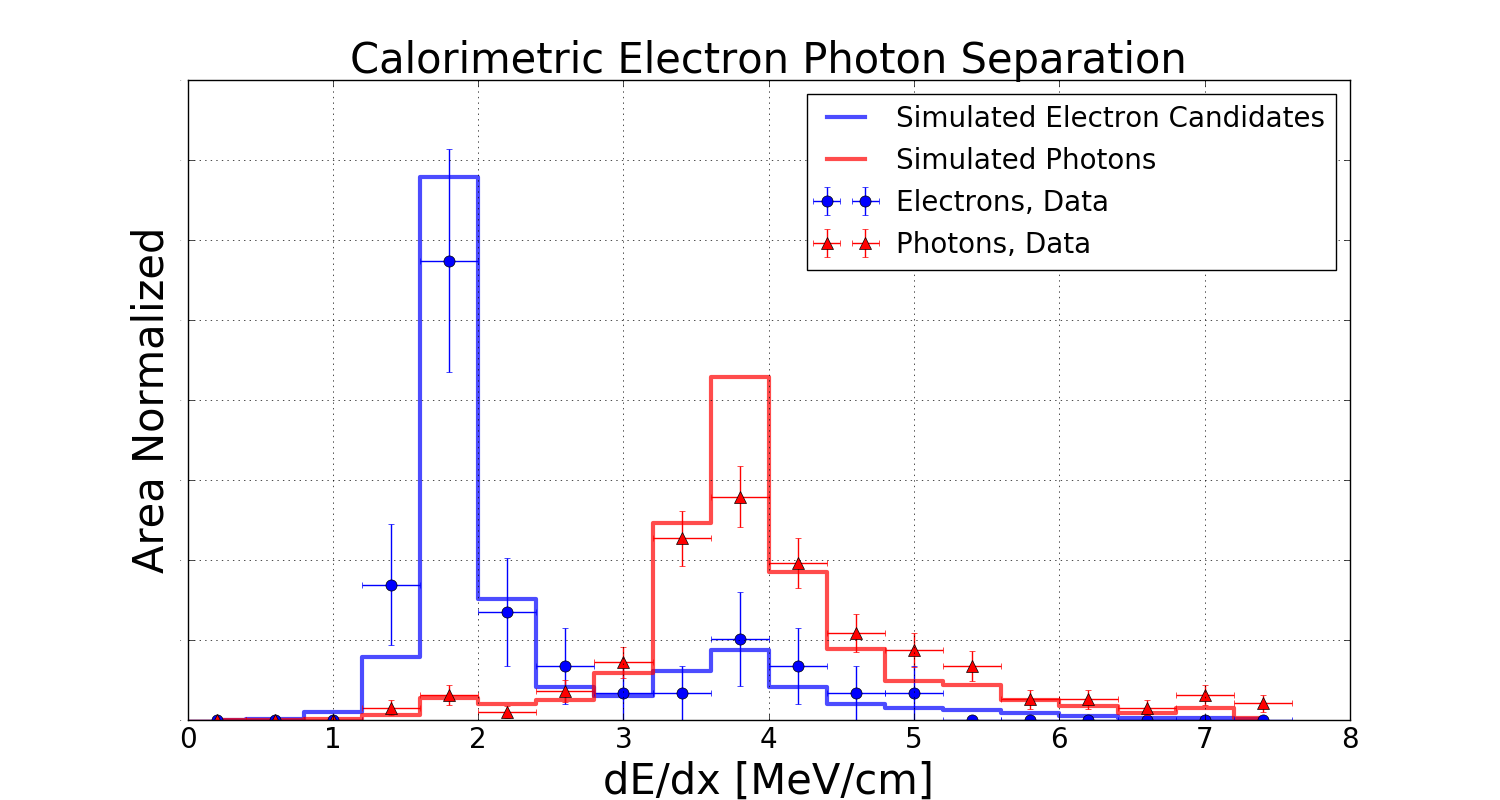
\includegraphics[width=0.95\textwidth]{emshower_figures/median_dedx.png}
  \caption[Calorimetric dE/dx Distribution]{The dE/dx distribution for electrons (blue) and gammas (red).  The solid blue curve, representing the simulation of electron dE/dx, includes a 20\% contaimination of gammas consistent with the results from Figure~\ref{fig:electron_landau}.}
  \label{fig:dEdx}
\end{figure}


Figure~\ref{fig:dEdx} represents the first demonstration of calorimetric separation of electrons and gammas in a LArTPC using neutrino events.  Despite the low statistics of the ArgoNeuT experiment, the electron and gamma separation using calorimetry is clearly validated. When a cut is made at 2.9 MeV/cm the efficiency of selecting electron candidate events in data is 76 $\pm$ 7\% with a 7 $\pm$ 2\% contamination from the gamma sample. Here, the uncertainties on the efficiency are estimated with the Feldman-Cousins method \cite{Feldman:1997qc} and are statistical only.  It must be noted, however, that the sample of electron candidates in this figure is not background subtracted.  The efficiency to select electrons with the same cut at 2.9 MeV/cm, estimated with the Monte Carlo, is 91\%.  This is consistent with the above measurement that 20 $\pm$ 15\% of the electron candidate sample, selected by topology only, is in fact gammas.


The value of the cut used above, 2.9 MeV/cm, is also somewhat arbitrary and must be determined uniquely for each analysis.  In this case, it is selected as the mid point between the two peaks of the distribution.  However, in an analysis targeting electron neutrinos the absolute normalization of the electron and gamma shower populations is crucial.  The desired purity of electrons must be balanced with the need to keep sufficient electron statistics.  An aggressive dE/dx cut, at 2.5 MeV/cm, effectively rejects gammas but also can remove a significant amount of electrons (removes 30\% of electron candidate events in data, 13\% of Monte Carlo electrons).  


As seen in figure~\ref{fig:electrons} and figure~\ref{fig:photons}, the high granularity of a LArTPC allows precision topological discrimination of gammas and electrons.  A purely topological cut produced a sample of electron events with an estimated 80 $\pm$ 15\% purity.  Further, full reconstruction of an event can improve gamma rejection.  For example, identification of two electromagnetic showers that reconstruct with an invariant mass consistent with the $\pi^0$ mass can remove both showers as electron candidates, even if there is not a gap present for one shower and the dE/dx cut fails.

The analysis in this chapter has shown that a metric based on the dE/dx deposition in the beginning part of the shower is valid method of separating electron-neutrino charged current events from gamma backgrounds. The full gamma background rejection capability of liquid argon detectors will be enhanced by adding to this a topological cut. This represents the first experimental proof of applying the calorimetric cut to separate electrons from gammas in a liquid argon detector using neutrino events.

One should note that the efficiency and misidentification rates presented here do not represent the full capability of liquid argon TPCs to discriminate gamma backgrounds from electron signals. The final separation power of LArTPCs leverages multiple identification techniques, of which calorimetry is just one.  Further, the exact efficiencies and misidentification rates depend heavily on the energy spectrum of the electromagnetic showers: the Compton scattering gammas, a major source of impurity, appear predominately at energies below 200 MeV.